\title{Warm-Up for March 28th, 2022}
\author{Dr. Jordan Hanson - Whittier College Dept. of Physics and Astronomy}
\date{\today}
\documentclass[12pt]{article}
\usepackage[a4paper, total={18cm, 27cm}]{geometry}
\usepackage{graphicx}
\usepackage{amsmath}
\usepackage{bm}
\def\rcurs{{\mbox{$\resizebox{.16in}{.08in}{
\includegraphics{ScriptR}}$}}}
\def\brcurs{{\mbox{$\resizebox{.16in}{.08in}{
\includegraphics{BoldR}}$}}}
\def\hrcurs{{\mbox{$\hat \brcurs$}}}
 
\begin{document}
\maketitle
\small
\section{Memory Bank}
\begin{enumerate}
\item Definition of voltage:
\begin{equation}
V(\mathbf{r}) = - \int_\mathcal{O}^{\mathbf{r}} \mathbf{E} \cdot d\mathbf{l} \label{eq:1}
\end{equation}
\item Work to place a point charge $Q$ with reference point at infinity:
\begin{equation}
U = QV(\mathbf{r})
\end{equation}
\item Field of a dipole (coordinate-free): 
\begin{equation}
\mathbf{E} = \frac{1}{4\pi\epsilon_0}\frac{1}{r^3}\left[ 3(\mathbf{p}\cdot\hat{\mathbf{r}})\hat{\mathbf{r}} - \mathbf{p}\right]
\end{equation}
\end{enumerate}

\section{Dipoles, Polarization, and Energy}

\begin{enumerate}
\item Show that the energy of an ideal dipole $\mathbf{p}$ in an electric field $\mathbf{E}$ is $U = -\mathbf{p} \cdot \mathbf{E}$. \textit{[Hint: use Eq. \ref{eq:1}].} \\ \vspace{2cm}
\item (a) Show that the interaction energy between two dipoles separated by a displacement $\mathbf{r}$ is 
\begin{equation}
U = \frac{1}{4\pi\epsilon_0}\frac{1}{r^3}\left[\mathbf{p}_1 \cdot \mathbf{p}_2 - 3(\mathbf{p}_1\cdot\hat{\mathbf{r}})(\mathbf{p}_2\cdot\hat{\mathbf{r}})\right] \label{eq:2}
\end{equation}
(b) Consider Fig. \ref{fig:1}.  If the dipoles are at right angles, show that Eq. \ref{eq:2} reduces to $U = -(3k/r^3) p_1 p_2$, with $k = 1/4\pi\epsilon_0$.
\end{enumerate}

\begin{figure}
\centering
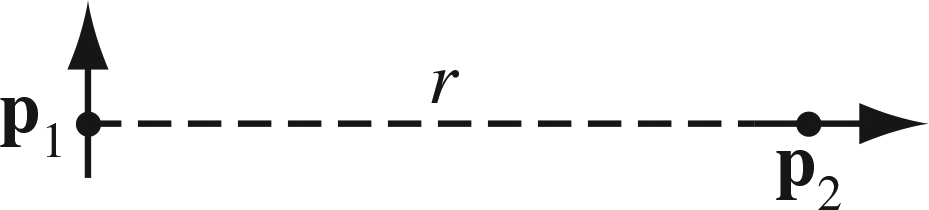
\includegraphics[width=0.3\textwidth]{figures/4_6.jpg}
\caption{\label{fig:1} Two orthogonal dipoles separated by a distance $r$.}
\end{figure}

\end{document}